\documentclass[11pt,a4paper,bibliography=totoc,listof=totoc]{scrartcl}

\usepackage[utf8]{inputenc}
\usepackage[T1]{fontenc}
\usepackage[ngerman]{babel}
\usepackage{lmodern}
\usepackage{microtype}
\usepackage[left=30mm,right=25mm,top=25mm,bottom=25mm]{geometry}
\usepackage{setspace}
\onehalfspacing

\usepackage{booktabs}
\usepackage{tabularx}
\usepackage{graphicx}
\usepackage{float}
\usepackage[labelfont=bf]{caption}
\usepackage{xcolor}
\usepackage{listings}
\usepackage[colorlinks=true,linkcolor=black,citecolor=black,urlcolor=blue]{hyperref}

\graphicspath{{figures/}}
\setlength{\emergencystretch}{2em}
\setcounter{tocdepth}{2}

\definecolor{codegreen}{rgb}{0,0.5,0}
\definecolor{codegray}{rgb}{0.45,0.45,0.45}
\definecolor{backcolour}{rgb}{0.96,0.96,0.94}
\lstdefinestyle{mystyle}{
    backgroundcolor=\color{backcolour},
    commentstyle=\color{codegreen},
    keywordstyle=\color{magenta},
    numberstyle=\tiny\color{codegray},
    basicstyle=\ttfamily\footnotesize,
    breaklines=true,
    keepspaces=true,
    numbers=left,
    numbersep=5pt,
    showstringspaces=false,
    tabsize=2
}
\lstset{style=mystyle}

\begin{document}

\hypersetup{pageanchor=false}
\begin{titlepage}
    \begin{center}
        \vspace*{1.5cm}
        {\large Berufliche Hochschule Hamburg -- Informatik\par}
        \vspace{0.6cm}
        {\large IT Security\par}
        \vspace{2.3cm}
        {\huge\bfseries Cross-Site Scripting und Cross-Origin Resource Sharing im Scheduler-Projekt\par}
        \vspace{1.2cm}
        {\Large Projektbericht\par}
    \end{center}

    \vfill

    \begin{tabular}{@{}ll@{}}
        \textbf{Projektgruppe:} & Arvid Freese\\
                               & Linus Paliga\\
                               & Tom Markmann\\
                               & Raik Ole Kannenberg\\[0.4cm]
        \textbf{Präsentation:}  & Hamburg, 10. Juni 2026\\
        \textbf{Berichtsstand:} & nach vollständigem XSS-Rollout auf \texttt{capstone-main}
    \end{tabular}
\end{titlepage}

\hypersetup{pageanchor=true}
\pagenumbering{Roman}
\section*{Abstract}
\begin{abstract}
  \noindent
  Dieser Projektbericht untersucht Cross-Site Scripting (XSS) und
  Cross-Origin Resource Sharing (CORS) anhand der realen
  Vue-/Spring-Boot-Anwendung \emph{Scheduler}. Die Themen wurden
  innerhalb der Gruppe aufgeteilt: Arvid Freese und Linus Paliga
  bearbeiteten XSS, Tom Markmann und Raik Ole Kannenberg CORS. Nach
  der Herleitung der theoretischen Grundlagen wurde das
  Scheduler-Repository systematisch auf relevante Datenflüsse,
  Ausgabesenken und Sicherheitskonfigurationen geprüft. Für beide
  Themen entstanden anschließend lokale Live-Demos.

  Die XSS-Analyse identifizierte eine reale
  Stored-DOM-XSS-Schwachstelle. Datenbankbasierte
  Veranstaltungsnamen, Gruppenbezeichnungen und Reservierungslabels
  wurden in mehreren Kalenderansichten an den Standardrenderer der
  Bibliothek \texttt{vue-cal} übergeben, der Event-Titel und -Inhalte
  als HTML rendert. Die Schwachstelle wurde durch eigene Event-Slots
  mit Vue-Interpolation strukturell behoben. Zum Berichtsstand ist
  dieser Fix auf \texttt{capstone-main} in allen relevanten
  Kalenderansichten ausgerollt; nach erneuter Prüfung besteht kein
  bekanntes aktuelles XSS-Risiko dieser Art.

  Die Spring-API besaß im untersuchten Ausgangsstand keine pauschale
  CORS-Freigabe. Die normale lokale Anwendung vermeidet
  Cross-Origin-Aufrufe über den Vite-Proxy. Für die Demo wurde im
  separaten Security-Branch bewusst eine unsichere globale
  Origin-Freigabe ergänzt und anschließend einer festen Allowlist
  gegenübergestellt. Unabhängig davon bleiben konkrete Verbesserungen
  erforderlich: \texttt{/files/**} ist zu breit öffentlich
  freigegeben, Keycloak verwendet für den Web-Client eine
  Wildcard-Origin sowie nicht benötigte OAuth-Flows, und das Frontend
  setzt trotz Bearer-Token-Authentifizierung \texttt{credentials:
  include}. Der Bericht leitet daraus priorisierte, direkt auf
  Scheduler-Dateien bezogene Maßnahmen ab.
\end{abstract}

\newpage
\tableofcontents
\newpage

\pagenumbering{arabic}
\section{Einleitung}
\label{sec:einleitung}

\subsection{Motivation}

Webanwendungen verarbeiten fortlaufend Daten aus Formularen,
Datenbanken, APIs und dem Browserkontext. Zwei zentrale
Sicherheitsgrenzen sind dabei die Trennung von Daten und ausführbarem
Code sowie die Trennung verschiedener Web-Origins. XSS verletzt die
erste Grenze: Ein eigentlich als Text gedachter Wert wird als HTML
oder JavaScript interpretiert. CORS steuert die zweite Grenze: Ein
Server kann dem Browser erlauben, Antworten auch fremden Origins
zugänglich zu machen.

Der Scheduler eignet sich als praxisnahes Untersuchungsobjekt, weil
er zahlreiche nutzerkontrollierbare Stammdaten und Kalenderansichten,
ein Vue-Frontend, eine Spring-Boot-API und Keycloak zur
Authentifizierung kombiniert. Ein Fehler an der Ausgabegrenze kann
dadurch im Browser eines eingeloggten Nutzers ausgeführt werden. Eine
zu breite Origin-Freigabe kann wiederum die durch die Same-Origin
Policy vorgesehene Lesesperre aufheben.

\subsection{Zielsetzung und Leitfragen}

Ziel des Projekts war nicht eine generische Darstellung der beiden
Themen, sondern eine konkrete Sicherheitsprüfung des
Scheduler-Projekts mit nachvollziehbaren Live-Demos und umsetzbaren
Verbesserungen. Der Bericht beantwortet vier Leitfragen:

\begin{enumerate}
  \item Welche XSS- und CORS-relevanten Datenflüsse und
    Konfigurationen existieren im Scheduler?
  \item Welche Schwachstellen oder riskanten Konfigurationen lassen
    sich tatsächlich belegen?
  \item Wie können Ursache, Wirkung und Behebung lokal demonstriert werden?
  \item Welche Maßnahmen sollten auf \texttt{capstone-main} dauerhaft
    umgesetzt und getestet werden?
\end{enumerate}

\subsection{Abgrenzung und Berichtsstand}

Die Prüfung bezog sich auf getrackte Quell- und Konfigurationsdateien
aus \texttt{api/}, \texttt{web/}, Docker, Nginx und dem
Keycloak-Realm-Export \texttt{scheduler.json}. Die konkrete
Rendering-Stelle in \texttt{vue-cal} wurde zusätzlich in der
installierten Bibliothek untersucht. Produktive Systeme wurden nicht
aktiv angegriffen.

Der Bericht beschreibt den Stand nach dem vollständigen Rollout des
XSS-Fixes auf \path{capstone-main}. Die Demo-Setups wurden dagegen in
einem separaten, von \path{capstone-main} abgeleiteten
Security-Demobranch umgesetzt. Absichtlich schwache
CORS-Einstellungen, Umschaltlogik und Demo-Testdaten gehören
ausschließlich zu diesem Demonstrationsstand und nicht zum produktiven Fix.

\section{Theoretische Grundlagen}
\label{sec:grundlagen}

\subsection{Cross-Site Scripting}

XSS entsteht, wenn nicht vertrauenswürdige Daten eine Ausgabesenke
erreichen, die den Wert als HTML oder JavaScript interpretiert. Der
eingeschleuste Code läuft anschließend im Origin der legitimen
Anwendung und unterliegt damit nicht der Same-Origin-Sperre gegenüber
dieser Anwendung. Er kann sichtbare Inhalte lesen, die Oberfläche
verändern und Requests über den vorhandenen Anwendungskontext
auslösen. OWASP empfiehlt deshalb kontextgerechtes Output Encoding
und sichere Framework-Ausgabe als primäre Schutzmaßnahme~\cite{owaspXss}.

Die klassischen Varianten unterscheiden sich durch Herkunft und
Lebensdauer des Payloads:

\begin{itemize}
  \item \textbf{Stored XSS}: Der Payload wird persistent gespeichert
    und bei späteren Aufrufen erneut ausgeliefert.
  \item \textbf{Reflected XSS}: Der Payload stammt aus dem aktuellen
    Request und wird unmittelbar zurückgegeben.
  \item \textbf{DOM-based XSS}: Die unsichere Verarbeitung erfolgt im
    Browser, beispielsweise über \texttt{innerHTML}.
\end{itemize}

Der im Scheduler gefundene Fall kombiniert Stored und DOM-based XSS:
Der Wert liegt dauerhaft in der Datenbank, wird über die API geladen
und erst beim Rendern durch \texttt{vue-cal} als HTML in das DOM geschrieben.

\subsection{Quellen, Senken und sichere Ausgabe}

Eine \emph{Quelle} ist ein kontrollierbarer Datenursprung,
beispielsweise ein Veranstaltungsname, Gruppenname oder
Reservierungslabel. Eine \emph{Senke} ist eine Operation, die Daten
als aktiven Inhalt interpretiert. Typische Senken sind
\texttt{innerHTML}, Vue-\texttt{v-html}, \texttt{insertAdjacentHTML}
oder ein Bibliotheksrenderer mit vergleichbarem Verhalten.

Vue-Interpolation mit doppelten geschweiften Klammern escaped HTML
standardmäßig und erzeugt Text statt aktiver
DOM-Strukturen~\cite{vueSecurity}. Genau diese Eigenschaft wird beim
Scheduler-Fix genutzt:

\begin{lstlisting}[caption={Sichere Ausgabe eines Kalenderereignisses}]
<template v-slot:event="{ event }">
    <div class="vuecal__event-content">
        <strong>{{ event.title }}</strong>
        <div>{{ event.content }}</div>
    </div>
</template>
\end{lstlisting}

Eine Content Security Policy (CSP) ist eine zusätzliche
Schutzschicht, ersetzt aber nicht die Behebung der unsicheren
Senke~\cite{owaspCsp}. Serverseitige Validierung verbessert
Datenqualität und begrenzt Payloads, kann kontextgerechtes Escaping
ebenfalls nicht ersetzen.

\subsection{Same-Origin Policy und CORS}

Eine Origin besteht aus Schema, Host und Port. Deshalb sind
\texttt{http://localhost:8078} und \texttt{http://localhost:8079}
verschiedene Origins. Die Same-Origin Policy verhindert
grundsätzlich, dass JavaScript einer Origin Antworten einer fremden
Origin liest. Ein Request kann dabei teilweise trotzdem gesendet
werden; blockiert wird vor allem der Zugriff des Skripts auf die Antwort.

CORS ist die kontrollierte Lockerung dieser Browserregel. Der Server
liefert dafür unter anderem folgende Header~\cite{mdnCors}:

\begin{itemize}
  \item \texttt{Access-Control-Allow-Origin}: erlaubte lesende Origin,
  \item \texttt{Access-Control-Allow-Credentials}: Freigabe
    browserseitiger Credentials,
  \item \texttt{Access-Control-Allow-Methods}: erlaubte HTTP-Methoden,
  \item \texttt{Access-Control-Allow-Headers}: erlaubte Request-Header,
  \item \texttt{Access-Control-Expose-Headers}: für JavaScript
    lesbare Response-Header.
\end{itemize}

Requests mit beispielsweise \texttt{Authorization} oder
\texttt{Content-Type: application/json} lösen üblicherweise einen
Preflight-Request mit \texttt{OPTIONS} aus. CORS muss deshalb vor der
Spring-Security-Authentifizierung verarbeitet werden, da der
Preflight noch keine Benutzer-Credentials enthält~\cite{springCors}.

\subsection{CORS ist keine Authentifizierung}

CORS vergibt keine fachlichen Rechte und schützt eine API nicht vor
direkten Requests außerhalb des Browsers. Authentifizierung
beantwortet, wer ein Nutzer ist; Autorisierung beantwortet, was
dieser Nutzer tun darf. CORS beantwortet lediglich, ob fremdes
Browser-JavaScript eine Antwort lesen darf.

Ebenso wichtig ist die Abgrenzung beim Scheduler: Das Frontend setzt
den Bearer-Token explizit im \texttt{Authorization}-Header. Eine
fremde Webseite erhält diesen Token nicht automatisch allein durch
eine offene CORS-Konfiguration. Ein Token-Leak setzt eine zusätzliche
Schwachstelle voraus, etwa XSS, eine unsichere Token-Antwort oder
falsch eingesetzte Cookie-Authentifizierung.

\section{Projektvorgehen und Untersuchungsgegenstand}
\label{sec:vorgehen}

\subsection{Arbeitsteilung}

Die Bearbeitung wurde entlang der beiden Themen aufgeteilt:

\begin{table}[H]
  \centering
  \caption{Arbeitsteilung innerhalb der Projektgruppe}
  \begin{tabularx}{\textwidth}{lX}
    \toprule
    \textbf{Thema} & \textbf{Verantwortliche und Aufgaben}\\
    \midrule
    XSS & Arvid Freese und Linus Paliga: Grundlagen, Suche nach
    Quellen und Senken, Analyse der \texttt{vue-cal}-Schwachstelle,
    XSS-Demo und Fix\\
    CORS & Tom Markmann und Raik Ole Kannenberg: Grundlagen, Analyse
    von Spring Security, Vite, Keycloak und Datei-Endpunkten,
    CORS-Demo und sichere Konfiguration\\
    \bottomrule
  \end{tabularx}
\end{table}

Anders als in einem iterativen Issue-Prozess wurden zunächst die
theoretischen Grundlagen getrennt erarbeitet. Anschließend prüften
beide Teilgruppen den Scheduler aus ihrer jeweiligen Perspektive. Die
Ergebnisse wurden in den Markdown-Berichten
\texttt{xss-analyse-und-demo.md} und
\texttt{cors-analyse-und-demo.md} konsolidiert und für die gemeinsame
Präsentation zusammengeführt.

\subsection{Scheduler-Architektur}

Der untersuchte Scheduler verwendet Spring Boot 3.0.1 und Java 17 im
Backend sowie Vue 3 und Vite im Frontend. Die Authentifizierung
erfolgt über Keycloak; die API validiert Bearer-JWTs als OAuth2 Resource Server.

\begin{table}[H]
  \centering
  \caption{Lokale Komponenten und Origins}
  \begin{tabular}{lll}
    \toprule
    \textbf{Komponente} & \textbf{Adresse} & \textbf{Rolle}\\
    \midrule
    Keycloak & \texttt{http://localhost:8080} & Identitätsprovider\\
    Spring-API & \texttt{http://localhost:8079} & Backend und Datenzugriff\\
    Vue-Frontend & \texttt{http://localhost:8078} & reguläre Webanwendung\\
    PostgreSQL & \texttt{localhost:5432} & persistente Daten\\
    Demo-Seite & \texttt{http://localhost:5173} & fremde Origin für CORS-Demo\\
    \bottomrule
  \end{tabular}
\end{table}

Das Frontend ruft die API relativ über \texttt{/api/...} auf.
\texttt{web/vite.config.js} leitet diese Requests lokal an Port 8079
weiter. Aus Sicht des Browsers bleiben die normalen Requests damit
same-origin zu Port 8078.

\subsection{Prüfmethode}

Die Analyse kombinierte statische Quellcodeprüfung,
Konfigurationsvergleich und kontrollierte lokale Demonstrationen. Für
XSS wurden nutzerkontrollierbare Felder bis zu ihren Ausgabestellen
verfolgt und eigene sowie externe HTML-Senken gesucht. Für CORS
wurden Spring Security, Vite-Proxy, Frontend-Requests,
Keycloak-Web-Origins, Nginx und öffentliche Datei-Endpunkte geprüft.

Die weiteren relevanten Entwicklungsbranches wurden ebenfalls auf das
VueCal-Muster geprüft; die ursprüngliche Schwachstelle ist dort
vorhanden. Der dauerhafte Fix wurde ausschließlich auf
\path{fix/vue-cal-xss-safe-rendering} mit Commit \texttt{08567da9}
umgesetzt und geprüft, und zwar ohne Demo-Umschaltung und ohne schwache
CORS-Konfiguration. Er ist bereit für den Merge in
\texttt{capstone-main}. Sämtliche anderen zum Berichtsstand geprüften
Remote-Branches weisen das ursprüngliche anfällige VueCal-Muster
weiterhin auf. Der Demo-Stand
\path{origin/its-xss-cors-security-break} behält bewusst sichere und
unsichere Varianten für den direkten Vergleich.

\section{XSS-Analyse und Behebung}
\label{sec:xss}

\subsection{Gefundene Stored-DOM-XSS-Schwachstelle}

Im eigenen Frontend-Code wurden keine direkten produktiven
Verwendungen von \texttt{v-html}, \texttt{innerHTML},
\texttt{insertAdjacentHTML} oder \texttt{eval} gefunden. Die
relevante Senke lag in der Drittbibliothek \texttt{vue-cal} in
Version \texttt{\^{}4.8.1}. Deren Standardrenderer behandelt
\texttt{event.title} und \texttt{event.content} als HTML.

Mehrere Scheduler-Ansichten übergaben datenbankbasierte Werte an
genau diese Felder, ohne einen eigenen Event-Slot zu definieren.
Besonders relevant waren folgende Komponenten:

\begin{itemize}
  \item \texttt{ReserveTimeslot.vue}: Reservierungslabel und
    Veranstaltungsname als \texttt{title},
  \item \texttt{AssignmentView.vue}: Veranstaltungs- und Gruppenname
    als \texttt{title} beziehungsweise \texttt{content},
  \item \texttt{EditIncompleteStateAvailabilities.vue}: Gruppenname
    als \texttt{content},
  \item \texttt{TimeSlotCalendarView.vue}: Verwendung des
    Standardrenderers und HTML-Strings für Statusicons.
\end{itemize}

Die bereits vorhandene Datei \texttt{ScheduleOverview.vue} zeigte das
sichere Gegenmuster: Sie definierte eigene \texttt{event}-Slots und
gab Titel, Inhalte und Annotationen über Vue-Interpolation aus.

\subsection{Konkreter Datenfluss und Risiko}

Der nachgewiesene Datenfluss verlief über eine persistente Quelle und
eine DOM-Senke:

\begin{center}
  \texttt{Eingabefeld / Import} $\rightarrow$ \texttt{Datenbank}
  $\rightarrow$ \texttt{API} $\rightarrow$
  \texttt{event.title/content} $\rightarrow$ \texttt{vue-cal innerHTML}
\end{center}

Ein harmloser lokaler Nachweis verwendete einen Wert der Form:

\begin{lstlisting}[caption={Lokaler XSS-Demo-Payload}]
XSS Demo <img src=x onerror="alert('XSS Demo')">
\end{lstlisting}

Das nicht vorhandene Bild löst den \texttt{onerror}-Handler aus. Der
Alert beweist lediglich Codeausführung. Realistisch könnte
eingeschleuster Code sichtbare Planungsdaten lesen, UI-Inhalte
manipulieren oder API-Requests im Kontext des eingeloggten Nutzers
auslösen. Das Risiko wird dadurch erhöht, dass
\texttt{web/src/App.vue} die Keycloak-Instanz als
\texttt{window.\$keycloak} verfügbar macht und der Access Token
zusätzlich im Vuex-Session-State liegt.

\subsection{Struktureller Fix}

Die Schwachstelle wurde nicht durch eine Payload-Blacklist behoben,
sondern durch Entfernung der unsicheren Ausgabesenke. Alle relevanten
\texttt{VueCal}-Instanzen mit nutzer- oder datenbankkontrollierten
Werten besitzen zum Berichtsstand eigene Event-Slots. Titel, Inhalte
und Statusinformationen werden darin als Text oder als strukturierte
UI-Elemente gerendert.

Der Demo-Stand \path{origin/its-xss-cors-security-break}
demonstriert den Unterschied exemplarisch mit zwei Komponenten:

\begin{itemize}
  \item \texttt{ReserveTimeslot.vue}: ursprünglicher Standardrenderer
    für die unsichere Demo,
  \item \texttt{ReserveTimeslotSafe.vue}: eigener
    \texttt{v-slot:event} mit \texttt{\{\{ event.title \}\}}.
\end{itemize}

\path{web/.env.xss-safe}, die Umschaltung in \path{web/src/router.js}
und die npm-Skripte \path{dev:xss-safe} beziehungsweise
\path{build:xss-safe} sind reine Demo-Artefakte. Auf
\texttt{capstone-main} ist der sichere Renderer direkt in den
regulären Ansichten umgesetzt; eine Laufzeitumschaltung zurück zur
anfälligen Variante ist dort nicht vorhanden. Die Umsetzung ist in
Commit \texttt{3742df35} mit der Nachricht
\texttt{fix: render VueCal events safely} dokumentiert.

\subsection{Bewertung nach dem Rollout}

Nach dem vollständigen Rollout und einer erneuten Prüfung aller
relevanten Kalenderansichten auf \texttt{capstone-main} besteht dort
kein bekanntes aktuelles XSS-Risiko über den
\texttt{vue-cal}-Standardrenderer. Sämtliche anderen zum
Berichtsstand geprüften Remote-Branches enthalten Commit
\texttt{3742df35} nicht und weisen das ursprüngliche anfällige
VueCal-Muster weiterhin auf. Diese Aussage bedeutet nicht, dass
zukünftige Änderungen automatisch sicher bleiben. Neue Bibliotheken,
neue Kalenderansichten oder eine spätere Verwendung von
\texttt{v-html} können dieselbe Schwachstellenklasse erneut
einführen.

\subsection{Verbleibende Schutzmaßnahmen}

Für nachhaltigen Schutz sind folgende Ergänzungen sinnvoll:

\begin{itemize}
  \item Security-Regressionstests, die typische Payloads in jeder
    Kalenderansicht als Text erwarten,
  \item serverseitige Längen- und Fachvalidierung für Namen, Labels,
    Annotationen und Freitextfelder,
  \item eine produktionsgerechte CSP ohne unnötiges \texttt{unsafe-inline},
  \item regelmäßige Prüfung von Dependency-Updates und Bibliotheksrenderern,
  \item Entfernung unnötiger globaler Token-Zugriffe wie
    \texttt{window.\$keycloak}.
\end{itemize}

\section{CORS-Analyse und Verbesserungen}
\label{sec:cors}

\subsection{Ausgangssituation der Spring-API}

Im Ausgangsstand von \texttt{capstone-main} war keine explizite Spring-CORS-Konfiguration vorhanden. Es gab weder \texttt{@CrossOrigin} noch eine \texttt{CorsConfigurationSource}, einen \texttt{CorsFilter} oder \texttt{http.cors()}. Direkte Cross-Origin-Antworten der API waren damit für fremdes Browser-JavaScript standardmäßig nicht lesbar.

Für die normale lokale Anwendung ist dies funktional unproblematisch. Die Vite-Konfiguration proxyt relative \texttt{/api}-Requests von Port 8078 an die API auf Port 8079. Der Browser sieht nur die Frontend-Origin. CORS wird erst sichtbar, wenn eine separate Seite, etwa auf Port 5173, die API direkt anspricht.

\subsection{Bewusst unsichere Demo-Konfiguration}

Der Branch \path{its-xss-cors-security-break} ergänzt für die Live-Demo eine Spring-CORS-Bean vom Typ \path{CorsConfigurationSource}. Die unsichere Variante akzeptiert mit \texttt{allowedOriginPatterns("*")} jede Origin und erlaubt gleichzeitig Credentials. Zusätzlich werden sämtliche üblichen Methoden und alle Header global für \texttt{/**} freigegeben.

\begin{lstlisting}[caption={Bewusst unsichere CORS-Demo, nicht für Produktion}]
config.setAllowedOriginPatterns(List.of("*"));
config.setAllowCredentials(true);
config.setAllowedMethods(List.of(
    "GET", "POST", "PUT", "PATCH", "DELETE", "OPTIONS"));
config.setAllowedHeaders(List.of("*"));
source.registerCorsConfiguration("/**", config);
\end{lstlisting}

Diese Konfiguration spiegelt praktisch jede anfragende Origin und hebt die Browser-Lesesperre global auf. Sie ist kein Bestandteil des produktiven XSS-Fixes und darf nicht nach \texttt{capstone-main} übernommen werden.

\subsection{Sichere Vergleichskonfiguration}

Die sichere Demo-Variante erlaubt ausschließlich das reguläre lokale Frontend:

\begin{lstlisting}[caption={Restriktive lokale Vergleichskonfiguration}]
config.setAllowedOrigins(List.of("http://localhost:8078"));
config.setAllowCredentials(false);
\end{lstlisting}

Eine dauerhafte CORS-Konfiguration sollte nur eingeführt werden, wenn ein echtes Cross-Origin-Frontend benötigt wird. Dann müssen Origins aus umgebungsspezifischen Properties stammen, Methoden und Header auf den tatsächlichen Bedarf begrenzt und Routen möglichst selektiv registriert werden. Da der Scheduler Bearer-Tokens explizit im \texttt{Authorization}-Header sendet, ist \texttt{allowCredentials(true)} für den aktuellen API-Flow nicht erforderlich.

\subsection{Öffentliche Datei-Endpunkte}

Die wichtigste CORS-nahe, aber eigenständige Schwachstelle liegt in \path{api/src/main/java/com/frostbear/scheduler/conf/SecurityConfiguration.java}. Der Matcher

\begin{lstlisting}
requestMatchers("/files/**").permitAll();
\end{lstlisting}

macht nicht nur bewusst tokenisierte Download-Links öffentlich, sondern auch den Voll-Export \texttt{GET /files/planningperiod/\{id\}/download} sowie mehrere Endpunkte zur Token-Erzeugung im \texttt{FileController}. CORS schützt diese Daten nicht vor direktem Zugriff. Die Demo zeigt lediglich zusätzlich, dass eine breite CORS-Freigabe die Antwort auch für fremdes Browser-JavaScript lesbar macht.

Die Regel sollte auf tatsächlich öffentliche Token-Downloads begrenzt werden. Voll-Exporte und Token-Erzeugung müssen authentifiziert, rollenbasiert autorisiert und auf die konkrete Planungsperiode beziehungsweise Person beschränkt werden.

\subsection{Keycloak- und Frontend-Konfiguration}

Der Realm-Export \texttt{scheduler.json} enthält für den Web-Client eine zu breite Konfiguration:

\begin{itemize}
    \item \texttt{webOrigins: ["*"]},
    \item \texttt{implicitFlowEnabled: true},
    \item \texttt{directAccessGrantsEnabled: true}.
\end{itemize}

Zusätzlich setzt der Realm \texttt{sslRequired} auf \texttt{none} und deaktiviert den Brute-Force-Schutz. Der OAuth 2.0 Security Best Current Practice rät vom Implicit Grant und vom Resource Owner Password Credentials Grant ab~\cite{rfc9700}. Für den Scheduler-Web-Client sollten konkrete Origins, Authorization Code Flow mit PKCE, TLS außerhalb der lokalen Entwicklung und aktivierter Login-Schutz verwendet werden.

\texttt{web/src/shared/http-client.js} setzt bei jedem Request \texttt{credentials: 'include'}, obwohl die API mit einem expliziten Bearer-Token arbeitet. Der Wert sollte auf \texttt{same-origin} oder \texttt{omit} reduziert werden, solange keine Cookie-basierte API-Sitzung benötigt wird. Dies verhindert, dass spätere Cookies unbeabsichtigt an Cross-Origin-Ziele gesendet werden.

\subsection{Bewertung}

Die Spring-API besaß im sicheren Ausgangsstand keine klassische Allow-All-CORS-Lücke. Das aktuelle Risiko entsteht aus benachbarten Konfigurationen: zu breite öffentliche Datei-Endpunkte, Keycloak-Wildcards, nicht benötigte OAuth-Flows und unnötige Credential-Übermittlung. Werden diese Punkte mit einer später versehentlich global aktivierten CORS-Freigabe kombiniert, wächst die Angriffsfläche erheblich.

\section{Live-Demos und technische Umsetzung}
\label{sec:demo}

\subsection{XSS-Demo}

Die XSS-Demo stellt denselben persistent gespeicherten Wert in einer
anfälligen und einer sicheren Kalenderansicht gegenüber. Der Test
\path{api/src/test/java/com/frostbear/scheduler/demo/XssDemoSetupTest.java}
bereitet eine vorhandene lokale Planungsperiode mit reproduzierbaren
Demo-Daten vor. Die zugehörige Gradle-Aufgabe \path{prepareXssDemo}
und die Property \path{xssDemoPlanningPeriodId} erlauben die gezielte Auswahl.

Die unsichere Ansicht übergibt das Event vollständig an den
Standardrenderer von \texttt{vue-cal}. Die sichere Ansicht
\texttt{ReserveTimeslotSafe.vue} definiert einen eigenen Event-Slot.
Über \texttt{VITE\_XSS\_SAFE\_RESERVATION\_VIEW} und die
Router-Umschaltung kann für die Präsentation zwischen beiden
Darstellungen gewechselt werden.

Der entscheidende Vergleich ist nicht ein unterschiedlicher Payload,
sondern dieselbe gespeicherte Eingabe:

\begin{enumerate}
  \item Unsichere Ansicht öffnen: Der Browser interpretiert den Wert
    als HTML und der lokale Alert erscheint.
  \item Sichere Ansicht öffnen: Der vollständige Payload bleibt
    sichtbar, wird aber nur als Text dargestellt.
  \item Ursache im Code zeigen: Standardrenderer mit HTML-Senke
    gegenüber eigenem Slot mit Vue-Interpolation.
\end{enumerate}

\subsection{CORS-Demo}

Die CORS-Demo verwendet vier lokale Komponenten: Keycloak und
PostgreSQL, die Spring-API auf Port 8079, das reguläre Vue-Frontend
auf Port 8078 sowie die separate Angreifer-Demo aus
\texttt{cors/index.html} auf Port 5173.

Die Seite ruft den öffentlichen Planungsperioden-Export direkt auf
und versucht, die Antwort als Datei zu lesen. Der Vergleich zeigt:

\begin{enumerate}
  \item Ohne passende CORS-Freigabe oder mit fester Allowlist
    blockiert der Browser den Lesezugriff der Origin \texttt{localhost:5173}.
  \item Mit der bewusst unsicheren globalen Freigabe kann die fremde
    Seite die Antwort lesen und den Download auslösen.
\end{enumerate}

\begin{figure}[H]
  \centering
  \begin{minipage}[t]{0.48\textwidth}
    \centering
    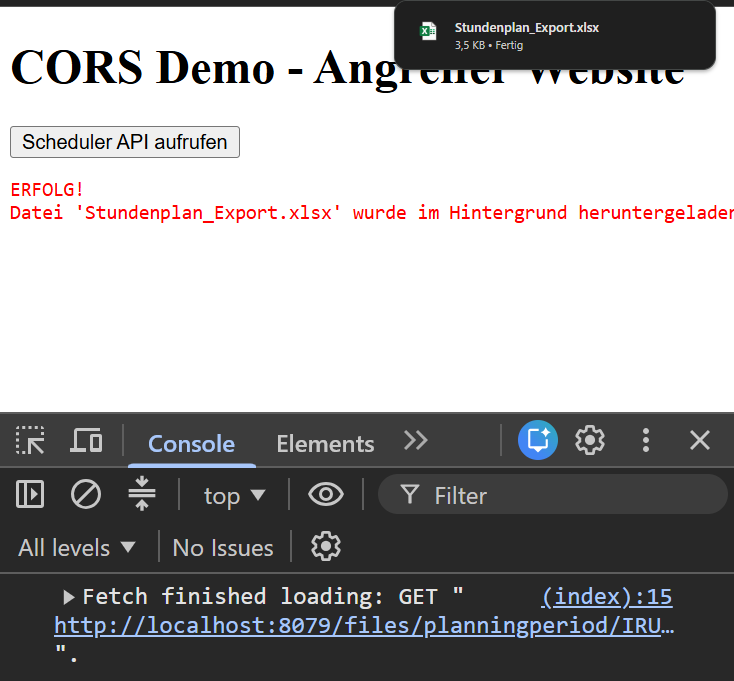
\includegraphics[width=\linewidth]{cors-unsecure}
    \caption*{Unsichere globale Freigabe: Antwort ist lesbar.}
  \end{minipage}
  \hfill
  \begin{minipage}[t]{0.48\textwidth}
    \centering
    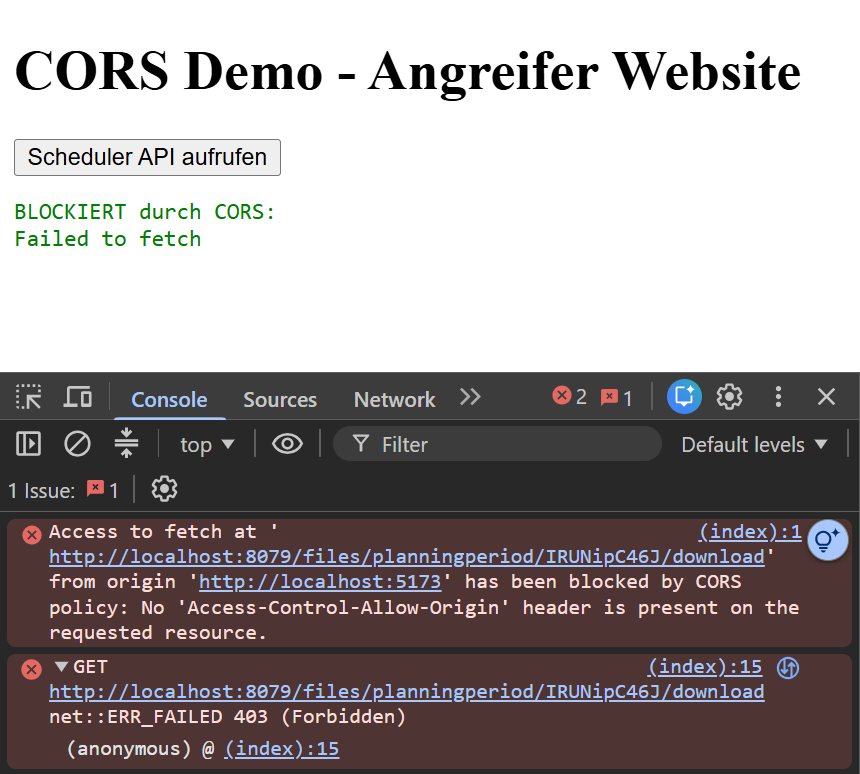
\includegraphics[width=\linewidth]{cors-secure}
    \caption*{Feste Allowlist: Demo-Origin wird blockiert.}
  \end{minipage}
  \caption{Gegenüberstellung der lokalen CORS-Demo}
  \label{fig:cors-demo}
\end{figure}

\subsection{Aussagekraft und Grenzen}

Die Demos beweisen jeweils einen klar abgegrenzten Mechanismus. Der
XSS-Alert beweist Codeausführung im Scheduler-Origin, aber noch keine
konkrete Datenexfiltration. Der CORS-Dateidownload beweist, dass eine
fremde Origin eine öffentliche Antwort lesen kann, aber noch keinen
Token-Diebstahl.

Insbesondere wird der Bearer-Token des Scheduler-Frontends nicht
automatisch durch \texttt{allowCredentials(true)} an die Demo-Origin
übertragen. Ein vollständiger Account-Takeover würde einen
zusätzlichen Fehler voraussetzen, etwa die nachgewiesene XSS-Klasse
vor ihrem Fix, eine unsichere Token-Antwort oder eine spätere
Cookie-basierte Authentifizierung mit fehlerhaftem CORS.

\section{Bewertung und priorisierte Maßnahmen}
\label{sec:massnahmen}

\subsection{Ergebnisübersicht}

\begin{table}[H]
  \centering
  \caption{Bewertung zum Berichtsstand nach XSS-Rollout}
  \small
  \begin{tabularx}{\textwidth}{l l X}
    \toprule
    \textbf{Bereich} & \textbf{Status} & \textbf{Begründung}\\
    \midrule
    VueCal Stored DOM XSS & behoben & Eigene Event-Slots und
    Vue-Interpolation sind auf \texttt{capstone-main} vollständig
    ausgerollt; erneute Prüfung ohne aktuellen Befund.\\
    Eigene Vue-HTML-Senken & kein Befund & Keine produktive direkte
    Verwendung von \texttt{v-html}, \texttt{innerHTML} oder
    vergleichbaren Senken in \texttt{web/src}.\\
    Spring API-CORS & kein Allow-All-Befund & Ohne Demo-Konfiguration
    keine explizite globale CORS-Freigabe; normale Entwicklung nutzt
    den Vite-Proxy.\\
    \texttt{/files/**} & hoch & Voll-Exporte und Token-Erzeugung
    liegen unter einer globalen \texttt{permitAll}-Regel.\\
    Keycloak Web-Client & hoch & Wildcard-Web-Origin und nicht
    benötigte beziehungsweise veraltete OAuth-Flows.\\
    Security-Regression & ausbaufähig & Spezifische automatisierte
    XSS-, CORS- und Autorisierungstests fehlen im regulären Stand.\\
    \bottomrule
  \end{tabularx}
\end{table}

\subsection{Priorität 1: Öffentliche Dateioberfläche begrenzen}

Die pauschale Freigabe von \texttt{/files/**} sollte durch getrennte
Regeln ersetzt werden. Nur ausdrücklich öffentliche, ausreichend
zufällige und möglichst zeitlich begrenzte Token-Downloads dürfen
ohne Login erreichbar sein. Folgende Endpunkte müssen mindestens
authentifiziert und fachlich autorisiert werden:

\begin{itemize}
  \item \texttt{GET /files/planningperiod/\{id\}/download},
  \item sämtliche \texttt{POST /files/create/...}-Endpunkte,
  \item \texttt{POST /files/get-or-create-ics-token}.
\end{itemize}

\subsection{Priorität 2: XSS-Fix durch Tests absichern}

Der ausgerollte Fix sollte mit Komponenten- oder End-to-End-Tests
gegen Regression geschützt werden. Für jede \texttt{VueCal}-Ansicht
wird ein Event mit HTML- und Event-Handler-Zeichenfolge gerendert.
Der Test muss bestätigen, dass der String als Text sichtbar bleibt
und kein DOM-Element aus dem Payload entsteht. Ergänzend sollte CI
nach neuen Verwendungen von \texttt{v-html}, \texttt{innerHTML} und
ähnlichen Senken suchen.

\subsection{Priorität 3: Keycloak und OAuth härten}

In \path{scheduler.json} sind konkrete Frontend-Origins statt
\texttt{*} zu hinterlegen. Implicit Flow und Direct Access Grants
sollten für den SPA-Web-Client deaktiviert, der Authorization Code
Flow mit PKCE verwendet und der Brute-Force-Schutz aktiviert werden.
Außerhalb lokaler Entwicklung muss TLS erzwungen werden.

\subsection{Priorität 4: CORS nur bei fachlichem Bedarf aktivieren}

Solange Frontend und API über denselben Origin beziehungsweise
Reverse Proxy erreichbar sind, ist keine globale API-CORS-Freigabe
nötig. Falls Cross-Origin-Zugriff eingeführt wird, sollte
\texttt{SecurityConfiguration.java} eine properties-basierte
Allowlist mit blockierendem Default erhalten. Die Registrierung
sollte auf tatsächlich benötigte Routen begrenzt werden. Demo-Origins
wie \texttt{localhost:5173} dürfen ausschließlich in einem lokalen
Entwicklungsprofil vorkommen.

\subsection{Priorität 5: Zusätzliche Schutzschichten}

\begin{itemize}
  \item \texttt{credentials: 'include'} in
    \texttt{web/src/shared/http-client.js} auf \texttt{same-origin}
    oder \texttt{omit} reduzieren.
  \item CSP im produktiven Reverse Proxy oder Backend einführen und
    zunächst im Report-Only-Modus testen.
  \item Freitextfelder serverseitig auf fachlich sinnvolle Längen und
    Werte validieren.
  \item \texttt{window.\$keycloak} entfernen oder den globalen
    Zugriff mindestens reduzieren.
  \item Dependency- und Security-Checks für npm und Gradle in CI integrieren.
  \item Die produktive Nginx-/Ingress-Konfiguration dokumentieren;
    die eingecheckte \texttt{nginx.conf} enthält derzeit keine
    \texttt{/api}-Proxy-Regel.
\end{itemize}

\section{Fazit}
\label{sec:fazit}

Die Untersuchung zeigt, dass Sicherheitsprobleme im Scheduler nicht
nur durch offensichtlich unsicheren eigenen Code entstehen. Die reale
XSS-Schwachstelle lag im Zusammenspiel aus kontrollierbaren
Datenbankwerten und dem komfortablen, aber für diese Daten
ungeeigneten Standardrenderer von \texttt{vue-cal}. Der strukturelle
Fix über eigene Event-Slots und Vue-Interpolation beseitigt die
Ursache. Nach dem vollständigen Rollout auf \texttt{capstone-main}
und erneuter Prüfung besteht kein bekanntes aktuelles XSS-Risiko dieser Art.

Bei CORS war die Ausgangslage differenzierter: Die Spring-API war
nicht pauschal für fremde Origins freigegeben und die normale lokale
Anwendung vermeidet Cross-Origin-Aufrufe über den Vite-Proxy. Erst
die bewusst unsichere Demo-Konfiguration machte den öffentlichen
Datei-Export für eine fremde Browser-Origin lesbar. Die Demo
verdeutlicht damit korrekt die Wirkung von CORS, darf aber nicht mit
Authentifizierung oder einem automatischen Token-Leak gleichgesetzt werden.

Der größte verbleibende Handlungsbedarf liegt in den angrenzenden
Schutzschichten. Die globale \texttt{/files/**}-Freigabe muss
begrenzt, die Keycloak-Konfiguration gehärtet und der XSS-Fix durch
Regressionstests abgesichert werden. CORS sollte weiterhin
blockierend bleiben, solange kein fachlicher Cross-Origin-Bedarf
existiert. Die zentrale Erkenntnis aus beiden Themen ist gleich:
Sicherheitsgrenzen müssen explizit kontrolliert werden. Nutzerdaten
gehören an eine Textausgabegrenze; fremde Origins erhalten nur die
minimal erforderliche Lesefreigabe.


\clearpage
\bibliographystyle{plain}
\bibliography{Quellen}

\clearpage
\appendix
\section{Anhang}
\label{sec:anhang}

\subsection{Zentrale Projektartefakte}

\begin{table}[H]
\centering
\caption{Relevante Artefakte für Analyse und Reproduktion}
\small
\begin{tabularx}{\textwidth}{lX}
\toprule
\textbf{Artefakt} & \textbf{Pfad}\\
\midrule
Gemeinsame Präsentation & \path{XSS-CORS-Praesentation.pptx}\\
XSS-Analyse & \path{xss/xss-analyse-und-demo.md}\\
CORS-Analyse & \path{cors/cors-analyse-und-demo.md}\\
CORS-Demo-Seite & \path{cors/index.html}\\
CORS-Screenshots & \path{cors/Cors secure.png}, \path{cors/Cors unsecure.png}\\
Security-Demobranch & \path{its-xss-cors-security-break}\\
XSS-Demo-Setup & \path{api/src/test/java/com/frostbear/scheduler/demo/XssDemoSetupTest.java}\\
Sichere Demo-Ansicht & \path{web/src/admin/views/data-admin/PlanningPeriodCrud/ReserveTimeslotSafe.vue}\\
Spring Security & \path{api/src/main/java/com/frostbear/scheduler/conf/SecurityConfiguration.java}\\
Datei-Endpunkte & \path{api/src/main/java/com/frostbear/scheduler/admin/controller/FileController.java}\\
Keycloak-Realm & \path{scheduler.json}\\
Frontend-HTTP-Client & \path{web/src/shared/http-client.js}\\
Vite-Proxy & \path{web/vite.config.js}\\
\bottomrule
\end{tabularx}
\end{table}

\subsection{Prüfliste für zukünftige Änderungen}

\begin{enumerate}
    \item Enthält jede neue \texttt{VueCal}-Ansicht einen eigenen sicheren Event-Slot?
    \item Werden nutzerkontrollierte Werte ausschließlich über Interpolation als Text ausgegeben?
    \item Gibt es neue Verwendungen von \texttt{v-html}, \texttt{innerHTML}, Raw HTML, Markdown-Renderern oder HTML-Tooltips?
    \item Sind neue Freitextfelder serverseitig validiert und durch Rendering-Tests abgedeckt?
    \item Ist eine neue CORS-Origin fachlich erforderlich und umgebungsspezifisch konfiguriert?
    \item Bleiben CORS-Methoden, Header und Routen auf das Minimum begrenzt?
    \item Ist jeder neue \texttt{/files}-Endpunkt ausdrücklich authentifiziert und autorisiert oder bewusst als öffentlicher Token-Download dokumentiert?
    \item Werden Keycloak-Web-Origins und OAuth-Flows bei Änderungen erneut geprüft?
\end{enumerate}


\end{document}
